
\section{Extending Drift for enterprise use}
\label{sec:ephemeris}

The effects of ``big data'' problems on information technology organizations have been well-documented.
Whether managing huge online presences, performing large-scale scientific experimentation and simulation,
or ingesting dense streaming data, these organizations face the challenge of converting vast stores of
data to actionable information.  Some of the specific problems faced in the application domain, however,
also manifest themselves in the management of enterprise data stores and sources.  For instance,
computational scientists and enterprise application developers both encounter ``siloed data'', where
domain boundaries restrict awareness about what potentially useful data may exist.
``Write-once-read-never'' issues, where data generation/collection rates outpace analysis and integration
processes, occur in both realms, as simulations generate petabytes of data per day and as documents
relating to design and testing processes accumulate over time, eventually succumbing to bit-rot.

We anticipate the integration of enterprise data stores and sources, once considered the exclusive
province of ``the IT shop'', with data analysis capabilities developed for use in application domains.
An example of this is the mining of employee safety incident data to reveal previously unknown trends and
correlations.  A service-based integration can also provide benefits in the opposite direction.  For
organizations which develop and maintain their own toolsets to support their work processes (such as
software libraries for high-performance computing tasks), making raw and analyzed data outputs available
in regular, extensible, and composable ways can improve productivity, accelerate the solution of new
problems and reduce reinvention of the wheel.

Drift includes specialized low-overhead publish/subscribe interfaces which are necessary for its HPC
role, but are not suitable for enterprise integration.  We are using an Enterprise Service Bus to provide
a service-oriented, discoverable, and general interface to Drift.

\newcommand{\eph}{Drift\xspace}

\begin{figure}
\centering{
  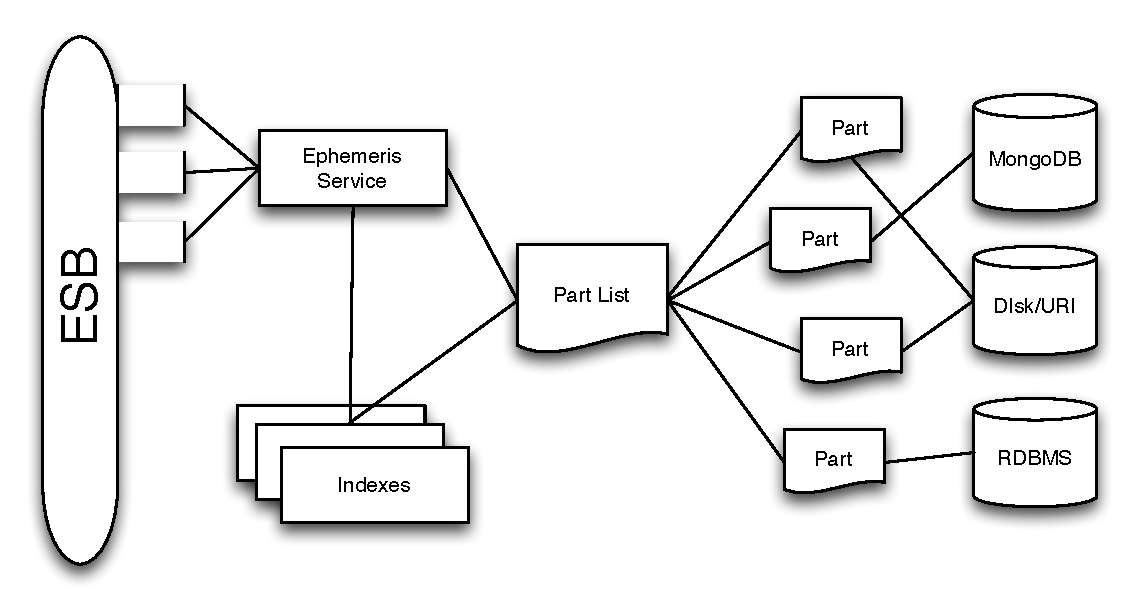
\includegraphics[width=5in]{figs/ep3}
}
\caption{Depiction of system-level relationship between Drift, the ESB, and other ESB services.}
\label{fig:eph}
\end{figure}

\subsection{Enterprise Data Fusion Services}


Drift was originally targeted at HPC and cloud environments, with specialized, low-overhead
publish/subscribe interfaces suited to their requirements.  While those kinds of considerations are
appropriate and necessary in a research software environment, they make integration into larger software
architectures very challenging.  Service-oriented architectures and software-as-a-service models adopted
in the pursuit of enterprise application integration have provided traction on these problems for
business applications.  The growing importance of metadata, Big Data problems, and coupled computations
on heterogeneous platforms is driving the development of research software whose SOA-style encapsulation
promises benefits outside their application domains\textemdash{}if the integration challenges can be
overcome.

We have explored the feasibility of such integration, using the data fusion and flexible indexing
capabilities of Drift as a test case. Our goal is to create an enterprise service with well-defined
endpoints, discovery and introspection capabilities.  We also want to make possible the construction of
more complex service-based offerings which make use of Drift service endpoints.

Given this goal, we have pursued an Enterprise Service Bus (ESB) approach using the open-source Mule
ESB~\cite{mule-esb}, extending Drift as a component called Ephemeris\cite{enterprise14:_patric_m} (Figure~\ref{fig:eph}).  Also, we have built \emph{Connectors} (integration units defined in the Mule
development framework) which will make \eph services available on a deployed Mule ESB.  The Connectors
mediate service requests to a separately running instance using a REST API.  The \eph instance will at
the same time be servicing application clients using its high-performance publish/subscribe interfaces.
In this manner, any service deployed on the ESB will be able to interact with the data fusion facilities
provided by \eph, using fused data defined by applications which have no coupling with the ESB.  This
integration will also provide benefits in the opposite direction: business processes attached to the ESB
will be able to define data fusions which will then be available for \eph application clients.

We have developed a Mule ESB Connector for Neo4j, so that fused data definitions and relationships can be
discovered and examined without interacting with the main service.  We believe this will be a powerful
new capability for integrating application data with enterprise data, making possible more holistic views
of an organization's data environment.  To explore the integration possibilities afforded by Mule's ESB,
we have also developed Connectors for certain internal Sandia services, as well as third-party tools used
internally at Sandia.  A test case for this is the Splunk connector (listing provided as
Appendix~\ref{sec:apx:splunk}.  Using this Connector and the ones provided for Sandia services such as
SAPLE and Drift, a Mule workflow can be constructed which retrieves information on up-to-date operational
information from a Splunk service, queries SAPLE for relevant employee contact information, and stores
the result data in a Drift instance.  Once stored in Drift, the data becomes ``fuse-able'' just as
any other data, providing end users with great flexibility in constructing data types for their own use
that reflect operational data.  



%%% Local Variables: 
%%% mode: latex
%%% TeX-master: "paper"
%%% End: 
